\DiaryEntry{Subband Coding}{2021-11-09}{Coding}

Working with signals in the temporal or spatial domain allowed us to use their correlation properties to develop techniques such as differential encoding and vector quantization. Working with signals in the frequency domain allowed us to use their spectral structure and develop transform coding approaches. In each case we stayed exclusively in one domain—either temporal and spatial or spectral.


In subband coding the signal is decomposed into frequency bands after which the temporal or spatial signal in each band can be separately encoded. This allows us to make use of the very different kinds of structures that exist in each band. The low frequency signals tend to be smoother allowing us to use sample to sample correlation if we wish. The high frequency signals tend to be sparse allowing us to use schemes more appropriate to sparse signals. Subband decomposition also permits the exploitation of both spectral and temporal limitations of human perception which can let us selectively ignore or discard components of the signal.


\subsection{Overview}

Subband coding uses the following structure.


\begin{figure}[H]
    \centering
    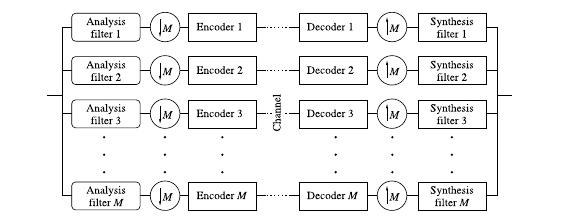
\includegraphics[scale=0.7]{images/2021-11-09-subband_01.png}
\end{figure}


\paragraph{Analysis.} The source output is passed through a bank of filters, called the analysis filter bank, which covers the range of frequencies that make up the source output. The passbands of the filters can be nonoverlapping or overlapping. The outputs of the filters are then subsampled; the filters are designed in such a way as to limit the bandwidth of the signals and therefore no information is lost due to subsampling. Of course, the filters need to be chosen accordingly.



\paragraph{Quantization and Coding.} Once the output of the filters has been subsampled, the output is encoded using one of several encod- ing schemes, including ADPCM, PCM, and vector quantization.

Along with the selection of the compression scheme, the allocation of bits between the subbands is an important design parameter. Different subbands contain differing amounts of information. Therefore, we need to allocate the available bits among the subbands according to some measure of the information content. There are a number of different ways we could distribute the available bits. 


\paragraph{Synthesis.} The quantized and coded coefficients are used to reconstruct a representation of the original signal at the decoder. First, the encoded samples from each subband are decoded at the receiver. These decoded values are then upsampled by inserting an appropriate number of $0$s between samples. Once the number of samples per second has been brought back to the original rate, the upsampled signals are passed through a bank of reconstruction filters. The outputs of the reconstruction filters are added to give the final reconstructed outputs.

\qed

We can see that the basic subband system is simple. The three major components of this system are the analysis and synthesis filters, the bit allocation scheme, and the encoding scheme. A substantial amount of research has focused on each of these components. Various filter bank structures have been studied in order to find filters that are simple to implement and provide good separation between the frequency bands.

The separation of the source output according to frequency also opens up the possibility for innovative ways to use compression algorithms. The decomposition of the source output in this manner provides inputs for the compression algorithms, each of which has more clearly defined characteristics than the original source output. We can use these characteristics to select separate compression schemes appropriate to each of the different inputs.

Human perception of audio and video inputs is frequency dependent. We can use this fact to design our compression schemes so that the frequency bands that are most important to perception are recon- structed most accurately. Whatever distortion there has to be is introduced in the frequency bands to which humans are least sensitive. We describe some applications to the coding of speech, audio, and images later in this chapter.


\subsection{Filterbanks}

Suppose we have a sequence $x_0, x_1, x_2 , \ldots$. We can divide this sequence into two subsequences: $x_0, x_2, x_4, \ldots$ and $x_1, x_3, x_5, \ldots$ using the scheme shown in the Figure below. This subsampling process is called \emph{downsampling} or \emph{decimation}.

\begin{figure}[H]
    \centering
    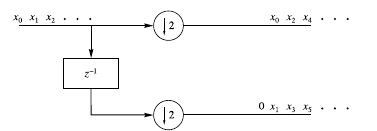
\includegraphics[scale=0.7]{images/2021-11-09-subband_02.png}
\end{figure}



The original sequence can be recovered from the two downsampled sequences by inserting $0$s between consecutive samples of the subsequences, delaying the top branch by one sample and adding the two together. Adding $0$s between consecutive samples is called upsampling. The reconstruction process is shown in the following Figure.

\begin{figure}[H]
    \centering
    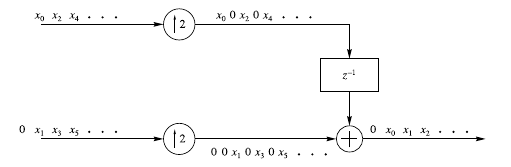
\includegraphics[scale=0.7]{images/2021-11-09-subband_03.png}
\end{figure}


A generalized filterbank system is shown in the following Figure: The source sequence $x[n]$ is fed into two \emph{analysis} filters $H_1(z)$ and $H_2(z)$ (input to the second filter is delayed by one), resulting into the signals $y_1[n]$ and $y_2[n]$. The signals are downsampled resulting in signals $v_1[n], v_2[n]$. Then the signals are encoding / decoded and upsampled, resulting in $u_1[n], u_2[n]$. After filtering with \emph{synthesis} $F_1(z), F_2(z)$, the first signal is delayed by one and then the signals are added.


\begin{figure}[H]
    \centering
    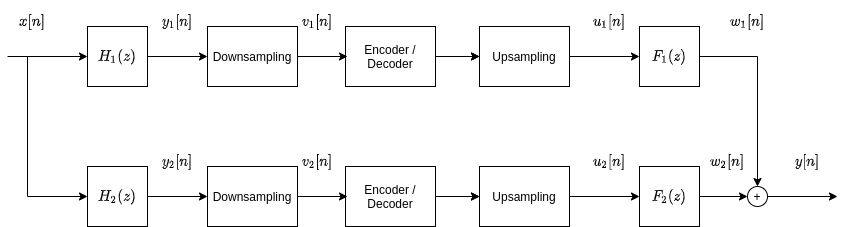
\includegraphics[scale=0.5]{images/2021-11-09-subband_04.png}
\end{figure}


We next investigate how up/down-sampling operates in the frequency domain.


\paragraph{Upsampling.} A signal $x[n]$ is upsampled, creating an output sequence $y[n]$ according to

\bee
y[n] = \begin{cases} x[n/2] & \text{ for $n$ even} \\ 0 & \text{otherwise} \end{cases}.
\eee


Between every signal point a zero is inserted and no information is lost. The z-transform of the output is given by

\bee
Y(z) = \sum_n y[n] z^{-n} = \sum_{n \text{even}} y[n] z^{-n} = \sum_{k} y[2k] z^{-2k} = \sum_{k} x[k] z^{-2k} = X(z^2)
\eee

For the DFT, we obtain $Y(e^{j \omega}) = X(e^{j 2 \omega})$, which corresponds to a compression of the spectrum. This is shown in the following Figure ($x[n]$ is black, $y[n]$ is red).

\begin{figure}[H]
    \centering
    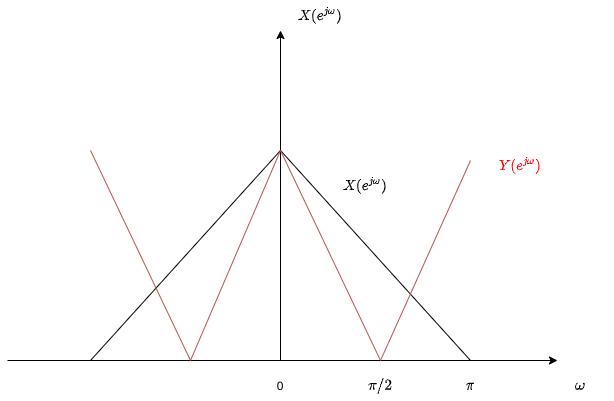
\includegraphics[scale=0.5]{images/2021-11-09-subband_05.png}
\end{figure}



\paragraph{Downsampling.} A signal $x[n]$ is downsampled, yielding a signal $y[n]$ given by

\bee
y[n] = x[2n]
\eee

Every second signal point is removed, therefore information is lost. The spectrum of the output signal can be shown to equal (proof omitted)

\bee
Y(e^{j \omega}) = \frac{1}{2} \left( X(e^{j \omega/2}) + X(e^{j(\omega - 2\pi)/2} \right)
\eee

This is shown in the following Figure ($x[n]$ is black, $y[n]$ is red). Note that when the bandwidth of the signal to be downsampled is larger than $\pi/2$, then aliasing is introduced and information is lost. This fact is shown in the lower part of the Figure.

\begin{figure}[H]
    \centering
    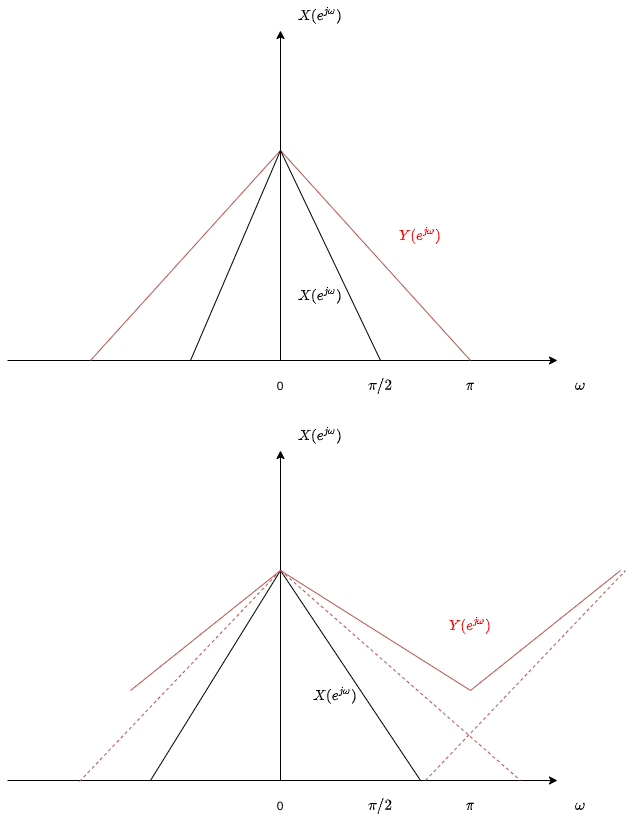
\includegraphics[scale=0.5]{images/2021-11-09-subband_06.png}
\end{figure}


Now consider a combined downsampling / upsampling system as shown below.


\begin{figure}[H]
    \centering
    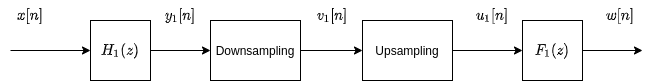
\includegraphics[scale=0.5]{images/2021-11-09-subband_07.png}
\end{figure}


Assume a low-pass signal $x[n]$. The first filter $H_1(z)$ must restrict the bandwidth of the input signal to $\pm \pi/2$. Then the downsampling will not remove information. After upsampling, the filter $F_1(z)$ will remove the ``repeated'' spectrum between $\pm \pi/2$ $\pm \pi$. However, this is not the only possible; we could also have a high-pass signal, restrict its bandwith using $H_1(z)$, down- and upsample it, and finally remove unwanted spectrum repetitions via the filter $F_1(z)$.

\qed


Coming back to our filter bank, we see that we have two upsampling / downsampling paths. In order to get perfect reconstruction, we have 4 filters (the 2 analysis filters $H_1(z), H_2(z)$ and the 2 synthesis filters $F_1(z), F_2(z)$) as ``design space'' so that $y[n] = x[n]$.


\subsection*{Perfect Reconstruction Filterbanks}


%%% Local Variables:
%%% mode: latex
%%% TeX-master: "journal"
%%% End:
